\documentclass[12pt,a4paper,bibliography=totocnumbered,listof=totocnumbered]{scrartcl}
\usepackage[ngerman]{babel}
\usepackage[utf8]{inputenc}
\usepackage{amsmath}
\usepackage{amsfonts}
\usepackage{amssymb}
\usepackage{graphicx}
\usepackage{fancyhdr}
\usepackage{tabularx}
\usepackage{geometry}
\usepackage{setspace}
\usepackage[right]{eurosym}
\usepackage[printonlyused]{acronym}
\usepackage{subfig}
\usepackage{floatflt}
\usepackage[usenames,dvipsnames]{color}
\usepackage{colortbl}
\usepackage{paralist}
\usepackage{array}
\usepackage{titlesec}
\usepackage{parskip}
\usepackage{acronym}
\usepackage{jurabib}
\jurabibsetup{
	authorformat=year,
	commabeforerest,
	ibidem=strict,
	citefull=first,
	see,
	titleformat=colonsep,
}
\usepackage{footmisc}
\usepackage[right]{eurosym}
\usepackage[subfigure,titles]{tocloft}
\usepackage[pdfpagelabels=true]{hyperref}

\usepackage{listings}
\lstset{basicstyle=\footnotesize, captionpos=b, breaklines=true, showstringspaces=false, tabsize=2, frame=lines, numbers=left, numberstyle=\tiny, xleftmargin=2em, framexleftmargin=2em}
\makeatletter
\def\l@lstlisting#1#2{\@dottedtocline{1}{0em}{1em}{\hspace{1,5em} Lst. #1}{#2}}
\makeatother

\geometry{a4paper, top=27mm, left=30mm, right=20mm, bottom=35mm, headsep=10mm, footskip=12mm}

\hypersetup{unicode=false, pdftoolbar=true, pdfmenubar=true, pdffitwindow=false, pdfstartview={FitH},
	pdftitle={Bachelorarbeit},
	pdfauthor={Fabian Wilms},
	pdfsubject={Bachelorarbeit},
	pdfcreator={\LaTeX\ with package \flqq hyperref\frqq},
	pdfproducer={pdfTeX \the\pdftexversion.\pdftexrevision},
	pdfkeywords={Bachelorarbeit},
	pdfnewwindow=true,
	colorlinks=true,linkcolor=black,citecolor=black,filecolor=magenta,urlcolor=black}
\pdfinfo{/CreationDate (D:20110620133321)}

\begin{document}

\titlespacing{\section}{0pt}{12pt plus 4pt minus 2pt}{-6pt plus 2pt minus 2pt}

% Kopf- und Fusszeile
\renewcommand{\sectionmark}[1]{\markright{#1}}
\renewcommand{\leftmark}{\rightmark}
\pagestyle{fancy}
\lhead{}
\chead{}
\rhead{\thesection\space\contentsname}
\lfoot{Generative Testerstellung für Microservice-Architekturen}
\cfoot{}
\rfoot{\ \linebreak Seite \thepage}
\renewcommand{\headrulewidth}{0.4pt}
\renewcommand{\footrulewidth}{0.4pt}

% Vorspann
\renewcommand{\thesection}{\Roman{section}}
\renewcommand{\theHsection}{\Roman{section}}
\pagenumbering{Roman}

% ----------------------------------------------------------------------------------------------------------
% Titelseite
% ----------------------------------------------------------------------------------------------------------
\thispagestyle{empty}
\begin{center}
	
\includegraphics[scale=0.5]{images/Hochschule_Muenchen_Logo.png}\\
	\vspace*{2cm}
	\Large
	\textbf{Fakultät für Informatik und Mathematik 07}\\
	\vspace*{2cm}
	\Huge
	\textbf{Bacheloararbeit}\\
	\vspace*{0.5cm}
	\large
	über das Thema\\
	\vspace*{1cm}
	\textbf{Generative Testerstellung für Microservice-Architekturenit}\\
	\vspace*{2cm}
	
	\vfill
	\normalsize
	\newcolumntype{x}[1]{>{\raggedleft\arraybackslash\hspace{0pt}}p{#1}}
	\begin{tabular}{x{6cm}p{7.5cm}}
		\rule{0mm}{5ex}\textbf{Autor:} & Fabian Wilms\newline holtkoet@hm.edu \\ 
		\rule{0mm}{5ex}\textbf{Prüfer:} & Prof. Dr. Ulrike Hammerschall \\ 
		\rule{0mm}{5ex}\textbf{Abgabedatum:} & xx.xx.2017 \\ 
	\end{tabular} 
\end{center}
\pagebreak

% ----------------------------------------------------------------------------------------------------------
% Abstract
% ----------------------------------------------------------------------------------------------------------
\setcounter{page}{1}
\onehalfspacing
\titlespacing{\section}{0pt}{12pt plus 4pt minus 2pt}{2pt plus 2pt minus 2pt}
\rhead{KURZFASSUNG}
\section{Kurzfassung}

Viele Softwareprojekte scheitern an fehlerhafter Kalkulation. Die Kosten werden meist viel zu gering angesetzt und sorgen für unzufriedene Kunden, geringe Erträge und fehlende Folgeaufträge. Doch warum ist das so?

Der größte Kostenfaktor sind Fehler im laufenden System. Diese Fehler zu beseitigen ist häufig eine große Herausforderung die viel Zeit, Personal und somit Geld kostet. Es gilt also, vor Auslieferung der Software eine entsprechende Qualität gewährleisten zu können.

Aus diesem Grund ist eine umfassende Testabdeckung ein sehr wichtiger Bestandteil in der Definition of Done der Landeshauptstadt München. Unit- und Integrations Tests sind fest in viele Entwicklungsprozesse integriert und finden besonders auch in agilen Entwicklerteams großen Zuspruch. Allerdings sind auch Tests finanzielle, wie auch zeitliche Kostenfaktoren.
Dennoch wird für Tests, trotz des Bewusstseins für die damit entstehenden Probleme, häufig viel zu wenig zeit eingeplant.

Um diesen problemen entgegen zu wirken wurde bei der LHM im vergangenen Jahr das Softwareprojekt Barrakuda entwickelt, welches anhand eines nach Domain Driven Design (DDD) aufgebauten Domänen-Modells Microservice Architekturen generieren kann. Die Idee: Software anhand von simplen Modellen generieren, um möglichst viel Zeit beim Entwickeln von "Boiler Plate"-Code einzsuparen, und die Software-Qualität nicht nur durch ersparte Entwicklungszeit, sondern auch durch homogene Projektstrukturen in allen generierten Systemen, und damit erhöhte Wartbarkeit, zu verbessern.

Im Rahmen dieser Bachelor-Arbeit soll die These geprüft werden, dass sich aus einem soclhen Modell genügend Informationen zum Testen eines Microservice-Frameworks extrahieren lassen, um eine ausreichende Testabdeckung für die generierten Services zu bieten.

Hierzu ist ein tieferes Verständnis der zu Generierung eingesetzten Sprache Barrakuda, welche von Martin Kurz in seiner Masterarbeit „Verbesserung des Softwareentwicklungsprozesses der Landeshauptstadt München durch modellgetriebene Softwareentwicklung“ entwickelt wurde, nötig. Diese wird in einem weiteren Abschnitt erklärt und anhand von Beispielen demonstriert. Um die Verbindung von Barrakuda zum DDD hervorzuheben, wird dies im weiteren Vorgehen näher beleuchtet.

Im zweiten Teilabschnitt werden dann die gängigsten Methoden und Praktiken, sowie Frameworks, die beim Testen von Microservice-Architekturen eingesetzt werden, identifiziert und weitere Anforderungsanalysen für diese durchgeführt, um die benötigte Bandbreite der generierten Tests abzugrenzen. Vorstellbare Testarten isnd Integrationstests, Unit-Tests und Smoke Tests.

Der letzte Schritt der Vorbereitung soll dann aus den zusammengetragenen Informationen festgestellen, für welches Framework ein generativer Ansatz zum Erstellen von Testfällen am sinnvollsten ist. Außerdem sollen eventuell benötigte Erweiterungen und/oder Änderungen von Barrakuda festgelegt werden, die für den generativen Ansatz von Nöten sind.

Im praktischen Teil der Arbeit werden dann zunächst einige Referenzimplementierungen umgesetzt, anhand derer im nächsten Teilschritt die Generierung der Tests, unter Zuhilfenahme von Barrakuda und den im vorherigen Teil festgelegten Änderungen, implementiert werden.

\vspace{-1,2em}
\titlespacing{\section}{0pt}{12pt plus 4pt minus 2pt}{-6pt plus 2pt minus 2pt}
\section*{Abstract}
Das ganze auf Englisch.
\pagebreak

% ----------------------------------------------------------------------------------------------------------
% Verzeichnisse
% ----------------------------------------------------------------------------------------------------------
% TODO Typ vor Nummer
\renewcommand{\cfttabpresnum}{Tab. }
\renewcommand{\cftfigpresnum}{Abb. }
\settowidth{\cfttabnumwidth}{Abb. 10\quad}
\settowidth{\cftfignumwidth}{Abb. 10\quad}

\titlespacing{\section}{0pt}{12pt plus 4pt minus 2pt}{2pt plus 2pt minus 2pt}
\singlespacing
\rhead{INHALTSVERZEICHNIS}
\renewcommand{\contentsname}{II Inhaltsverzeichnis}
\phantomsection
\addcontentsline{toc}{section}{\texorpdfstring{II \hspace{0.35em}Inhaltsverzeichnis}{Inhaltsverzeichnis}}
\addtocounter{section}{1}
\tableofcontents
%\pagebreak
\rhead{VERZEICHNISSE}
\listoffigures
%\pagebreak
\listoftables
%\pagebreak
\renewcommand{\lstlistlistingname}{Listing-Verzeichnis}
{\labelsep2cm\lstlistoflistings}
%\pagebreak

% ----------------------------------------------------------------------------------------------------------
% Abkürzungen
% ----------------------------------------------------------------------------------------------------------
\section{Abkürzungsverzeichnis}
\begin{acronym}[DDD] % längste Abkürzung steht in eckigen Klammern
	\acro{DDD}{Domain-Driven Design}
	\acro{LHM}{Landeshauptstadt München}
\end{acronym}
\newpage

% ----------------------------------------------------------------------------------------------------------
% Inhalt
% ----------------------------------------------------------------------------------------------------------
% Abstände Überschrift
\titlespacing{\section}{0pt}{12pt plus 4pt minus 2pt}{-6pt plus 2pt minus 2pt}
\titlespacing{\subsection}{0pt}{12pt plus 4pt minus 2pt}{-6pt plus 2pt minus 2pt}
\titlespacing{\subsubsection}{0pt}{12pt plus 4pt minus 2pt}{-6pt plus 2pt minus 2pt}

% Kopfzeile
\renewcommand{\sectionmark}[1]{\markright{#1}}
\renewcommand{\subsectionmark}[1]{}
\renewcommand{\subsubsectionmark}[1]{}
\lhead{Kapitel \thesection}
\rhead{\rightmark}

\onehalfspacing
\renewcommand{\thesection}{\arabic{section}}
\renewcommand{\theHsection}{\arabic{section}}
\setcounter{section}{0}
\pagenumbering{arabic}
\setcounter{page}{1}

% ----------------------------------------------------------------------------------------------------------
% Einführung und Motivation
% ----------------------------------------------------------------------------------------------------------
\section{Einführung und Motivation}

IT nimmt sowohl im privaten als auch geschäftlichen Alltag eine immer größere Rolle ein. Die Übernahme von Bereichen, die ehemals als nicht durch Computer austauschbar erachtet wurden, schreitet immer weiter fort. Doch dadurch steigen nicht nur bestehende Anforderungen an Software, sondern es entstehen auch neue Kriterien. Ganz abgesehen davon steigt die Komplexität von modernen Software-Systemen immens an.

Mit steigender Komplexität und höherer Nachfrage am Markt, sowie engen Zeitplänen für Projekte wird leider häufig aus Zeit- und Kostengründen auf Qualität nur geringfügig Rücksicht genommen. Zunächst verursacht eine gute Software-Qualität nämlich nur Mehrkosten. Personelle wie zeitliche. Die langfristige Sinnhaftigkeit bleibt dabei außen vor, aus der Vergangenheit wird nur selten gelernt.

Der Chaos Report von 2014 zeigt erschreckend wie viele IT-Projekte in der Versenkung verschwanden oder aber erst durch enorme Mehrkosten fertiggestellt werden konnten.

\vspace{1em}
\begin{minipage}{\linewidth}
	\centering
	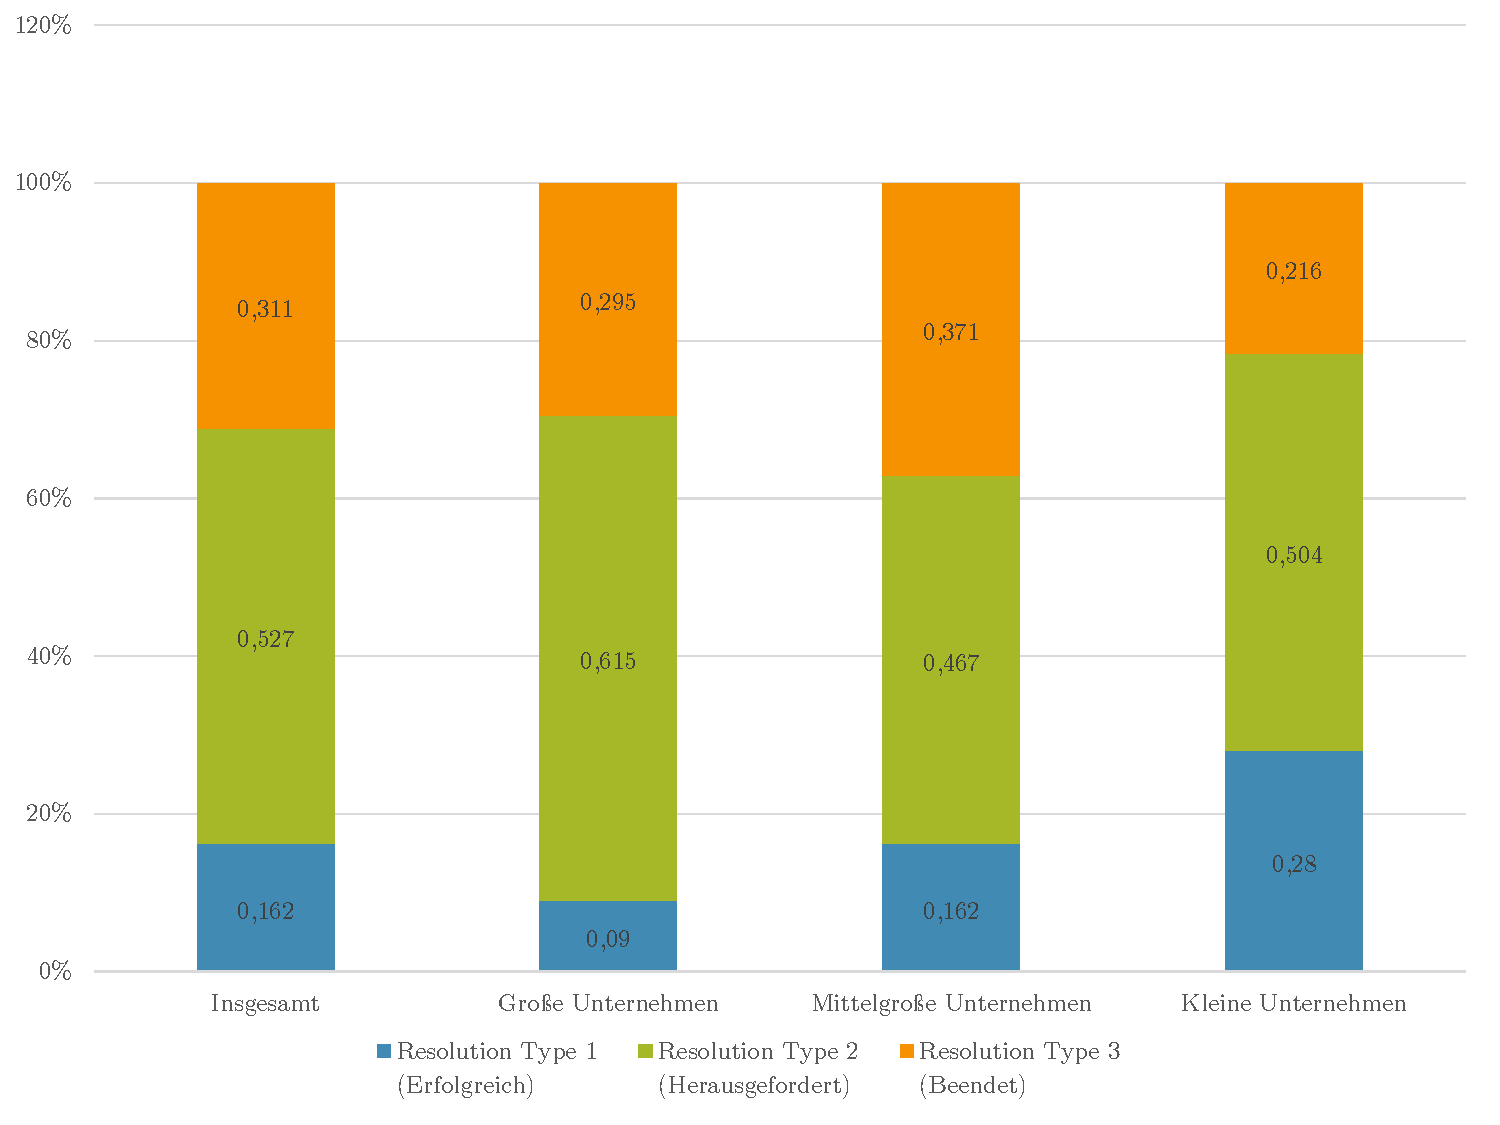
\includegraphics[width=0.9\linewidth]{images/dg_failed-projects.pdf}
	\captionof{figure}[Chaos Report 2014 Failure Statistics]{Chaos Report 2014 Failure Statistics \footcite[]{chaosreport}}
	\label{fig:dg_failed-projects}
\end{minipage}

Die Projekte wurden drei verschiedenen Klassen zugeteilt. RT1 entspricht einem erfolgreich abgeschlossenen Projekt, welches zeitlich und finanziell fertiggestellt wurde, sowie alle Features und Funktionalitäten die gefordert wurden enthält. RT2-Projekte wurden zu spät, zu teuer, und nicht mit allen Features ausgeliefert. RT3 sind abgebrochene Projekte.

Doch wie kommt es dazu, dass in derart vielen Projekten die festgelegten Ziele nicht ganz, oder sogar gar nicht erreicht werden? Es gibt unzählige Faktoren die dazu führen. Doch sind es einige die immer wieder in diesem Zusammenhang genannt werden. //TODO

Für die Größte Kostenexplosion sorgt jedoch das Bug-Fixing in Produktivsystemen. Wurde in den ersten Phasen eines Projekts nicht viel, oder kein Wert auf eine ausreichende Test-Abdeckung gelegt schaffen es viele Fehler in die Produktivsysteme der Hersteller. Doch werden diese Fehler erst im laufenden Betrieb beim Kunden festgestellt, ist es bereits zu spät. Robert N. Charette kritisiert eben dies in seinem Artikel \textit{Why Software Fails}.

\begin{quote}
	\begin{itshape}
	If the software coders don't catch their omission until final system testing--or worse, until after the system has been rolled out--the costs incurred to correct the error will likely be many times greater than if they'd caught the mistake while they were still working on the initial [...] process.\footcite{charette}
	\end{itshape}
\end{quote}

Ein Bericht der Kölner Beratungsfirma SQS zeigt dies anhand von gesammelten Zahlen aus Beratungsaufträgen. hier wird besonders deutlich wie viel es für ein Projekt bedeutet, frühzeitige Qualitätssicherung durchzusetzen. Und dazu zählt auch das testen von Software.

\vspace{1em}
\begin{minipage}{\linewidth}
	\centering
	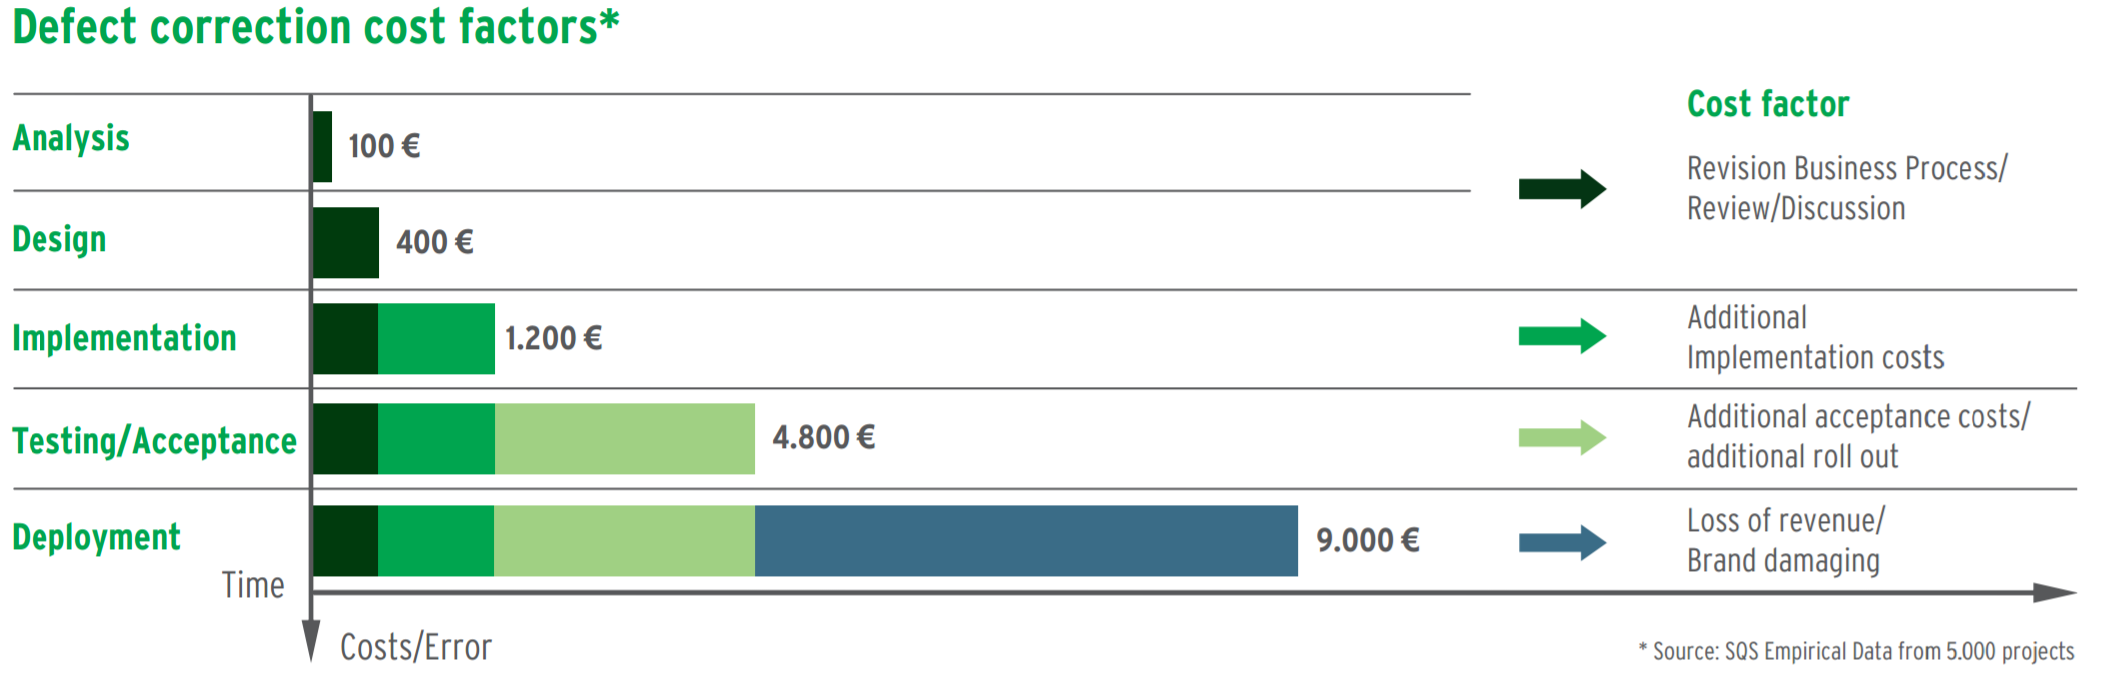
\includegraphics[width=0.9\linewidth]{images/img_sqs-defect-correction.PNG}
	\captionof{figure}[SQS Report Costs of Defect Correction]{SQS Report Costs of Defect Correction \footnotemark}
	\label{fig:img_sqs-defect-correction}
\end{minipage}
\footnotetext{\cite{sqsdefect}}

Es ist also eigentlich ganz einfach: Viel Zeit und Geld in gute Softwarequalität investieren und schon sollte das Projekt keine unvorhergesehenen Kosten verursachen. Doch so einfach ist es leider nicht.
Wie bereits am Anfang der Einleitung erwähnt stehen Projektleiter und seine Mitarbeiter unter hohem zeitlichen Druck. Und Tests kosten nun mal Zeit. Es entsteht in dieser Zeit aber kein messbarer Fortschritt am Produkt. Dies ist auch der Grund, weshalb das Testen bei Entwicklern nicht an oberster Stelle an den liebsten Aufgaben steht. Es kostet Zeit ohne erkennbaren Fortschritt zu erreichen.

Es muss also die Zeit, die für das entwickeln von Tests benötigt wird, reduziert werden, sowie mehr Zeit geschaffen werden, um für eine gute Softwarequalität zu sorgen. Diesen Ansatz verfolgt die Eigenentwicklung von it@M Barrakuda und deren Weiterentwicklung im Rahmen dieser Arbeit.

% ----------------------------------------------------------------------------------------------------------
% Architektur-Generierung für Software-Projekte
% ----------------------------------------------------------------------------------------------------------
\section{Architektur-Generierung für Software-Projekte}

\subsection{Barrakuda}

Im Rahmen seiner Master-Arbeit hat der Angestellte des Eigenbetriebs it@M der Landeshauptstadt München mithilfe von X-Text und X-Tend eine Sprache entwickelt, die es erlaubt, anhand eines Domänen-Ähnlichen Modells eine Microservice-Architektur zu generieren.

\subsubsection{Idee}

\subsubsection{Einführung}

\subsubsection{Verbindung zum Domain-driven Design}

\paragraph{Domain-driven Design in Microservices}

\paragraph{Umsetzung}

\subsubsection{Beispiel}

\subsubsection{Verbesserung der Software-Qualität bei der LHM mit Barrakuda}

% ----------------------------------------------------------------------------------------------------------
% Testen von Microservices
% ----------------------------------------------------------------------------------------------------------

\section{Testen von Microservices}

\subsection{Unterschiede zwischen Microservices und Monolith-Architekturen}

\subsection{Test-Strategien und deren Nutzen für Barrakuda}

\subsubsection{Bekannte Vorgehensweisen}

\subsubsection{Neue Vorgehensweisen}

\subsection{Frameworks zum Umsetzen von Test-Strategien für Barrakuda}

% ----------------------------------------------------------------------------------------------------------
% Anforderungen an generierte Tests
% ----------------------------------------------------------------------------------------------------------
\section{Anforderungen an generierte Tests}

\subsection{Anforderungen an generierte Tests}

\subsection{Notwendige Änderungen/Erweiterungen von Barrakuda}

% ----------------------------------------------------------------------------------------------------------
% Implementierung in Barrakuda
% ----------------------------------------------------------------------------------------------------------
\section{Implementierung in Barrakuda}

\subsection{Implementierung eines Referenz-Systems und dessen Tests}

\subsection{Übernahme der Referenz-Implementierung in Barrakuda}

% ----------------------------------------------------------------------------------------------------------
% Literatur
% ----------------------------------------------------------------------------------------------------------
\renewcommand\refname{Quellenverzeichnis}
\bibliographystyle{jurabib}
\bibliography{bibfile}
\pagebreak

% ----------------------------------------------------------------------------------------------------------
% Anhang
% ----------------------------------------------------------------------------------------------------------
\pagenumbering{Roman}
\setcounter{page}{1}
\lhead{Anhang \thesection}

\begin{appendix}
\section*{Anhang}
\phantomsection
\addcontentsline{toc}{section}{Anhang}
\addtocontents{toc}{\vspace{-0.5em}}

\section{Code-Fragmente}
Viel Beispiel-Code

\end{appendix}

\end{document}
